% Author: CSC Officers
\documentclass[11pt]{article}
\usepackage[margin=0.7in]{geometry}
\usepackage{listings}   %
\usepackage{needspace}  %
\usepackage{color}      %
\usepackage{ifthen}     % 
\usepackage{graphicx}   %
\usepackage{../includes/csc}        %
\usepackage{tikz}       %
\usetikzlibrary{shapes} %
\usepackage{tabularx}   % for helping matchtabular (matching questions)
\usepackage{textcomp}	% So our quotes in code don't look like shit
\usepackage{longtable}
\usepackage{multicol}
\usepackage[usenames,dvipsnames]{pstricks}
\usepackage{epsfig}
\setlength{\columnsep}{12em}

\lstset{ %
basicstyle=\footnotesize\ttfamily,       % the size of the fonts that are used for the code
numbers=left,                   % where to put the line-numbers
stepnumber=1,                   % the step between two line-numbers. If it's 1 each line will be numbered
numbersep=5pt,                  % how far the line-numbers are from the code
showspaces=false,               % show spaces adding particular underscores
showstringspaces=false,         % underline spaces within strings
tabsize=4,		                % sets default tabsize to 4 spaces
language=C,
upquote=true,
columns=fixed
}

\ifthenelse{\isundefined{\isAnswerKey}}
{
    \newenvironment{answer}{\large\lstset{basicstyle=\tiny\ttfamily}\color{white}}{}
}
{
    \newenvironment{answer}{\large\lstset{basicstyle=\large\ttfamily}\color{red}}{}
}

% ----- Start matchtabular definition -----
\newcounter{matchleft}
\newcounter{matchright}
\newenvironment{matchtabular}{%
  \setcounter{matchleft}{0}%
  \setcounter{matchright}{0}%
  \tabularx{\textwidth}{%
    >{\leavevmode\hbox to 1.5em{\stepcounter{matchleft}\arabic{matchleft}.}}X%
    >{\leavevmode\hbox to 1.5em{\stepcounter{matchright}\alph{matchright})}}X% 
    }%
}{\endtabularx}
% ----- End matchtabular definition -----

\title{CSCI-142 Exam 1 Review}
\author{Computer Science Community}
\date{\today}

\makeatletter
\let\thetitle\@title
\let\theauthor\@author
\let\thedate\@date
\makeatother

\begin{document}
\header

\begin{enumerate}

\section*{History and Evolution of Programming Languages}

	\item Explain the relationship between machine language, assembly language, and high level languages.\\
\begin{answer}
\small{\textbf{Machine language} is a set of instructions that is executed directly as-is by the computer's CPU itself. This is considered the lowest level representation of a computer program, and, while it is possible to program directly in machine code, it is highly tedious and error prone, making higher level languages favorable. Writing machine code is typically only done when troubleshooting a system or when implementing extreme optimization.\\
\textbf{Assembly language} is also considered a low-level programming language, and, in particular, assembly usually has a near 1:1 relationship between the assembly code and the architechure's machine code instructions. Assembly languages are specific to a computer's architechture - for example, assembly code you write for your phone (almost certainly) wouldn't work on your laptop. An example of an assembly language is MIPS. Programming in assembly language (and lower) is commonplace in embedded systems work.
\\
Finally, \textbf{high level languages} are, in general, designed to be portable across many different architechtures. What separates the high level languages from their lower level counterparts is that, due to this fact, they require compiling, which translates your high-level code into a form which the machine can understand (which varies by architechture.) When people talk about programming languages, they are most often referencing one of the high level languages, unless otherwise specified. High level languages include C and C++, Python, and Java.}
\end{answer}


\section*{Differences in Language Paradigms}

	\item \begin{enumerate}

\item List a difference between imperative/procedural programming and object-oriented programming.

\begin{answer}
In procedural programming, the program is a flat collection of global functions and variables. In object-oriented programming, functions and variables are grouped into classes, where they can be encapsulated from other classes.
\end{answer}


\item List a difference that functional programming has from procedural or object-oriented programming.

\begin{answer}
In functional programming, functions return values based solely on their input, and do not affect the state of any other data. Rather than programs being composed of statements executed in sequence, programs are composed of function applications which produce the desired output.
\end{answer}

\end{enumerate}


\section*{Programming In C}

	\item Explain the purpose of each of the following GCC options:
\begin{itemize}
	\item -o	\hspace{20mm}
		\begin{answer}
		Place output in a specific file.
		\end{answer}
	\item -c	\hspace{20mm}
		\begin{answer}
		Compile/assemble source files, but do not link them.
		\end{answer}
	\item -std	\hspace{17mm}
		\begin{answer}
		Specify a specific C standard to use during compilation.
		\end{answer}
	\item -Wall	\hspace{14mm}
		\begin{answer}
		Turn on all optional warnings.
		\end{answer}
	
\end{itemize}

\newpage
\section*{Modular Design and Development}

	\item For each of the following snippets of code, state whether it should be placed in the header file (\texttt{.h}) or the source file (\texttt{.c}).

\begin{enumerate}

\begin{tabular}{p{.25in}p{1.5in} p{4.5in}}
\item
&
{
\begin{lstlisting}[numbers=none]
struct Point
{
	double x;
	double y;
};
\end{lstlisting}
}
&
\begin{answer}
Either. If the fields of the type need to be accessed from other source files, it must be defined in the header; otherwise, it only needs to be defined in the source file and possibly forward-declared or \texttt{typedef}'d in the header.
\end{answer}
\\
\item
&
{
\begin{lstlisting}[numbers=none]
int main(int argc, char **argv)
{
	int x = run_some_function();
	printf("%d\n", x);
	return 0;
}
\end{lstlisting}
}
&
\begin{answer}
\hspace{2.5in}
Source
\end{answer}
\\
\item
&
{
\begin{lstlisting}[numbers=none]
int do_something_and_return(int x, int y)
{
	if (y != 0)
		return x*y + (x/y);
	else
		return x*y;
}
\end{lstlisting}
}
&
\begin{answer}
\hspace{2.5in}
Source
\end{answer}
\\
\item
&
{
\begin{lstlisting}[numbers=none]
int do_something_and_return(int x, int y);
void do_something(int x, int y);
\end{lstlisting}
}
&
\begin{answer}
\hspace{2.5in}
Header
\end{answer}
\\
\end{tabular}
\end{enumerate}

	\item Give an example of a header guard for a header file named \texttt{linkedlist.h}.

\begin{answer}
\begin{lstlisting}
#ifndef LINKEDLIST_H
#define LINKEDLIST_H

<code>

#endif
\end{lstlisting}
\end{answer}


\section*{Variables and Basic Data Types}

	\item List the 7 basic data types in C (not including the unsigned variants).

\begin{answer}
char, short, int, long, long long, float, double
\end{answer}

\newpage
\section*{Initialization and Coercion}

	\item There are at least two issues in the following code. What are they?

\begin{verbatim}
#include <stdio.h>

int main(void) {
    int numbers[] = { 3, 6, 4, 5, 14, 9 };
    int sum, i = 0;
    double average;
    for (; i < 6; ++i) {
        sum += numbers[i];
    }
    average = sum / 6;
    printf("%f", average);
    return 0;
}
\end{verbatim}

\begin{answer}
\begin{enumerate}
\item \texttt{sum} is not initialized to 0, so \texttt{sum} does not contain the actual sum of the numbers in the array.
\item Because \texttt{sum} and \texttt{6} are both of type \texttt{int}, integer division is performed, and \texttt{average} does not contain the expected average, but the floor of the average. Change that line of code to one of the following:
\begin{verbatim}
average = sum / 6.0;
\end{verbatim}
\begin{verbatim}
average = (double)sum / 6;
\end{verbatim}
\begin{verbatim}
average = sum / (double)6.0;
\end{verbatim}
\end{enumerate}
\end{answer}


\section*{Strings}
	\item If you want to store the string \texttt{``Hello, world!''} in the \texttt{str} variable in the following code, at least what value should \texttt{n} have? Why?
\begin{lstlisting}
int n;
...
char str[n];
\end{lstlisting}

\begin{answer}
It should at least have the value 14.
There are 13 characters in the string, and one place in the string is needed for the null terminator.
\end{answer}

\item What is the character literal for the null terminator?

\begin{answer}
\texttt{`\textbackslash0'}
\end{answer}


\pagebreak

\section*{Arrays}
	
	\item What is the issue with the code below? What is the result of the issue?

\begin{lstlisting}
int i, x;
int arr[10];
for (i=0; i < 10; ++i)
{
	scanf("%d", &x); // Reads a number from stdin and stores it in x
	arr[i] = x;
}

for (i=10; i >= 0; --i)
{
	printf("%d\n", arr[i]);
}
\end{lstlisting}
\begin{answer}
The second for loop starts at 10, not 9.
\texttt{arr[10]} is out of bounds, but since C doesn't check for this the behavior is undefined.
It might not actually crash at run time, it might just get whatever happens to be in memory at that location.
\emph{Scary}.
\end{answer}


\section*{I/O}

	\item There is a problem with the following code as written that will manifest itself for certain user input. Explain what this issue is and how to solve it.

\begin{verbatim}
#include <stdio.h>

int main(void) {
        const int BUF_SIZE = 256;
        char buf[BUF_SIZE];
        while (fgets(buf, BUF_SIZE, stdin)) {
                printf(buf);
        }
}
\end{verbatim}

\begin{answer}
If the user enters a string with a \texttt{\%} character, \texttt{printf} will try to interpret this string as a format string, which will fail as there are no other arguments to \texttt{printf} for it to format. To solve this issue, replace \texttt{printf(buf);} with \texttt{printf("\%s", buf);}.
\end{answer}


\pagebreak

\section*{Memory and Program Layout}

	\item \textbf{Memory and Program Layout}

Label the sections of the program in memory

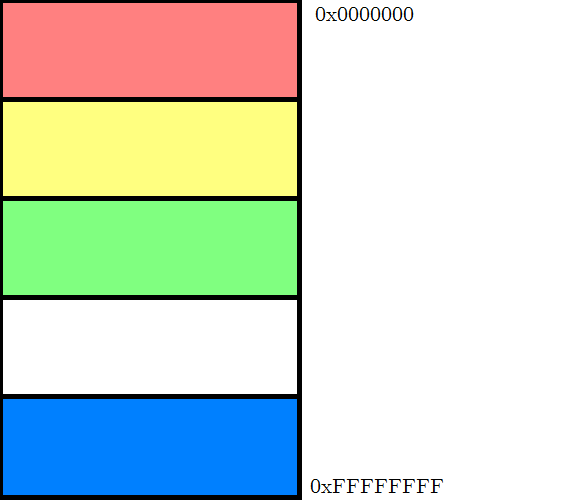
\includegraphics[width=50mm]{questions/programstructure.png}

\begin{answer}
red: text

yellow: data

green: heap

blue: stack
\end{answer}

\section*{C Pre-processor}

	\item What is the value of \texttt{i}?
\begin{verbatim}
#define THING1 40
#define THING2 32

#if THING1 < THING2
#define THING3 5
#elif THING2 < THING1
#define THING3 6
#else
#define THING3 7
#endif

int i = THING3;
\end{verbatim}
\begin{answer}
6
\end{answer}

\newpage
\section*{C Pointers}

	\item %
% NOTE: This question is meant to take up one full page
%	and includes all necessary spacing.
%


\begin{enumerate}
\item What does the following function do?

\begin{lstlisting}
int foo(int n, int *arr, int **bestp)
{
	int *start;
	int *end;
	int best = 0;
	*bestp = arr;
	
	for (start = arr; start < arr + n; ++start)
	{
		for (end = start; end < arr + n && *end == *start; ++end);
		if ((end - start) > best)
		{
			best = (end - start);
			*bestp = start;
		}
		start = end - 1;
	}
	
	return best;
}
\end{lstlisting}

\begin{answer}
Finds the longest sequence of identical integers in the given array.
Returns the length of the sequence and stores the pointer to the start of the sequence in \texttt{bestp}.
\end{answer}

\item Make a memory map of \texttt{foo}. Use the first value set to each variable in the map.

\begin{answer}
Stack: n, arr, bestp, start, end, best

Heap: *arr (size n), *bestp (size int)

start \rightarrow arr

end \rightarrow start

bestp \rightarrow arr
\end{answer}

\item Given the following code in \texttt{main}, write the code to call our \texttt{foo} function above.
Also write the code to output the result.
\begin{lstlisting}[numbers=none]
int main(int argc, char **argv)
{
	int n, i;
	int arr[] = {1, 1, 1, 2, 2, 2, 5, 5, 5, 5};

	// Write your code here

	return 0;
}
\end{lstlisting}

\begin{answer}
\begin{lstlisting}
int main(int argc, char **argv)
{
	int n = 10;
	int arr[] = {1, 1, 1, 2, 2, 2, 5, 5, 5, 5};

	int *res = NULL;

	int i;
	n = foo(n, arr, &res);

	for (i=0;i<n;++i)
	{
		printf("%d, ", res[i]);
	}
	puts("");
	return 0;
}
\end{lstlisting}
\end{answer}
\end{enumerate}


\pagebreak
\section*{Structs, Dynamic Storage}

	\item \begin{enumerate}
\item The following program compiles. Will it crash at run time? If so, on which line will it crash?

\begin{lstlisting}
#include <stdlib.h>
int main(int argc, char **argv)
{
	int *x = NULL;
	int *y = NULL;
	int *z = NULL;

	x = malloc(sizeof(int) * 10);
	y = malloc(20);
	x = malloc(sizeof(char) * 50);

	free(x);
	free(y);
	free(z);

	return 0;
}
\end{lstlisting}

\begin{answer}
No, it runs and terminates normally.
\texttt{free} will not do anything if the pointer passed to it is \texttt{NULL}.
\end{answer}

\item Does the above program have a memory leak? If so, where?

\begin{answer}
Yes, the first call to \texttt{malloc} is never freed.
\end{answer}
\end{enumerate}


\end{enumerate}
\end{document}

Topics for this exam:
	- History and Evolution of Programming Languages
	- Differences in Language Paradigms
	- Programming Environments
	- Modular Design and Development
	- C: Variables, basic data types
	- C: control structures, operators, arrays  YAWAR
	- C: basic I/O
	- C: basic CPP
	- The OS: memory, program layout
	- C: Functions, Structs, Strings			KATIE
	- Program Maintenance
	- C Pointers and Dynamic Storage			KATIE
